% \iffalse meta-comment
%
% Copyright 2025-2026 Michael E. Hammer
%
% This work may be distributed and/or modified under the
% conditions of the LaTeX Project Public License, either version 1.3
% of this license or (at your option) any later version.
% The latest version of this license is in
%   http://www.latex-project.org/lppl.txt
% and version 1.3 or later is part of all distributions of LaTeX
% version 2005/12/01 or later.
%
% This work has the LPPL maintenance status `maintained'.
% 
% The Current Maintainer of this work is Michael E. Hammer.
%
% This file is part of the "fhj-script bundle" and all files in that
% bundle must be distributed together.
%
% \fi
% \iffalse
%<package>\NeedsTeXFormat{LaTeX2e}[2023-11-01]
%<package>\ProvidesPackage{fhjcommon}
%<package>[2026-10-05 v4.3d Common macros for the FHJ bundle]
%
%<*driver>
\documentclass{ltxdoc}
\usepackage{fhjcommon}
\EnableCrossrefs
\CodelineIndex
\RecordChanges
\OnlyDescription % We only want the description
\begin{document}
    \DocInput{fhjcommon.dtx}
\end{document}
%</driver>
% \fi
%
% \GetFileInfo{fhjcommon.sty}
% \FHJProgram{DAT-25}
%
% \changes{v4.0}{2025/08/03}{Initial package version}
% \changes{v4.3}{2026/07/30}{Study programs moved to a data table registered via
%   \cs{FHJDefineProgram}; added Applied Computer Science, Business Informatics and
%   Cybersecurity and Ethical Hacking}
% \changes{v4.3}{2026/07/30}{\cs{FHJProgramLong} and \cs{FHJProgramShort} take an
%   optional \meta{code} that sets the study program inline}
% \changes{v4.3}{2026/07/30}{Removed \cs{FHJDATLong}, \cs{FHJDATShort}, \cs{FHJIMSLong}
%   and \cs{FHJIMSShort}}
% \changes{v4.3b}{2026/07/31}{\cs{FHJExHeaderScheduled} now forwards the type as the
%   optional argument to \cs{FHJExHeader}, so the exercise id is no longer overwritten
%   by the type}
%
% \title{The \textsf{fhjcommon} package\thanks{This document corresponds to
%       \textsf{fhjcommon}~\fileversion, dated \filedate.}}
% \author{Michael E. Hammer \\ \texttt{michael.hammer@fh-joanneum.at}}
%
% \maketitle
% 
% \begin{abstract}
% Collection of common macros for the FHJ bundle independent of a chosen
% document class.
% \end{abstract}
% 
% \tableofcontents
% 
% \section{Configuration}
% 
% \subsection{Used Packages}
% 
%    \begin{macrocode}
%<*package>
\RequirePackage{xstring}
\RequirePackage{ifthen}
\RequirePackage{calc}
%    \end{macrocode}
% 
% \section{Naming definitions}
% 
% \DescribeMacro{\FHJ}
% One goal of this package is to provide common naming definitions which can and should 
% be used in all documents which are created in the context of \textit{\FHJ}. This 
% includes the naming of the university (\cs{FHJ}), the study programs and their long 
% and short names.
% 
% \subsection{Study program specifics}
%
% \DescribeMacro{\FHJProgram}
% It is assumed that the documents which are generated are created in the context of
% a given study program. To set the study program for the given document use the macro
% as following:
%
% \begin{quote}
%   \cs{FHJProgram}\marg{code}
% \end{quote}
%
% This updates what \cs{FHJProgramLong} and \cs{FHJProgramShort} expand to -- the long
% and short name registered for \marg{code}. Passing an unregistered \marg{code} raises
% a package error listing the currently known codes. \cs{FHJProgram} also accepts
% \texttt{ITP}, which is not a study program but refers to the institute itself -- see
% the remark at the end of this subsection.
%
% \iffalse
\newcommand{\FHJ@CurrentLong}{}
\newcommand{\FHJ@CurrentShort}{}
\newcommand{\FHJProgram}[1]{%
  \ifthenelse{\equal{#1}{ITP}}{%
    \renewcommand{\FHJ@CurrentLong}{Institute for Information Technology+}%
    \renewcommand{\FHJ@CurrentShort}{\FHJInstitute}%
  }{%
    \@ifundefined{FHJProgram@#1@Long}{%
      \PackageError{\FHJ@PackageName}%
        {Unknown study program option: #1.\MessageBreak
         Known study programs are: \FHJ@ProgramList\MessageBreak
         (or ITP for the institute itself)}%
        {Register new study programs with \string\FHJDefineProgram\space
         before calling \string\FHJProgram, or check for a typo.}%
    }{%
      \renewcommand{\FHJ@CurrentShort}{\csname FHJProgram@#1@Short\endcsname}%
      \renewcommand{\FHJ@CurrentLong}{\csname FHJProgram@#1@Long\endcsname}%
    }%
  }%
}
% \fi
%
% \DescribeMacro{\FHJProgramLong} and \DescribeMacro{\FHJProgramShort}
% \cs{FHJProgramLong}\oarg{code} and \cs{FHJProgramShort}\oarg{code} expand to the long
% and short name of the currently set study program. Given the optional \oarg{code},
% they first call \cs{FHJProgram}\marg{code} -- switching the study program for the rest
% of the document -- and then expand to its long/short name; this is convenient for
% setting and using the study program name in a single place, without a separate
% \cs{FHJProgram} call beforehand.
%
% \iffalse
\newcommand{\FHJProgramLong}[1][]{%
  \ifthenelse{\equal{#1}{}}{}{\FHJProgram{#1}}%
  \FHJ@CurrentLong
}
\newcommand{\FHJProgramShort}[1][]{%
  \ifthenelse{\equal{#1}{}}{}{\FHJProgram{#1}}%
  \FHJ@CurrentShort
}
% \fi
%
% \DescribeMacro{\FHJDefineProgram}
% Study programs are registered in a small table, keyed by a \marg{code} that stays
% stable for a program's lineage while it may carry a year suffix marking when a given
% name \emph{first became official} (e.g. \texttt{IMS-26}) -- this is not a student
% cohort year. New codes are registered with
%
% \begin{quote}
%   \cs{FHJDefineProgram}\marg{code}\marg{short name}\marg{long name}
% \end{quote}
%
% \marg{code} may contain letters, digits and hyphens. The \marg{short name} is stored
% separately from \marg{code} on purpose -- a code's year suffix should not leak into
% the displayed short name, so e.g. both \texttt{DAT-22} and \texttt{DAT-25} use the
% short name \texttt{DAT}. For example
% \cs{FHJDefineProgram}\{AIM-27\}\{AIM\}\{Applied Computer Science\} registers
% \texttt{AIM-27} so that \cs{FHJProgram}\{AIM-27\} afterwards sets \cs{FHJProgramShort}
% to ``AIM'' and \cs{FHJProgramLong} to ``Applied Computer Science''. This is the
% intended extension point for future study programs: maintainers or downstream users
% can call \cs{FHJDefineProgram} for a new program without editing \cs{FHJProgram}
% itself, as long as the call happens before \cs{FHJProgram} is used. The code
% \texttt{ITP} is reserved for the institute (see below) and cannot be registered this
% way.
%
% \iffalse
\newcommand{\FHJ@ProgramList}{}
\newcommand{\FHJDefineProgram}[3]{%
  \ifthenelse{\equal{#1}{ITP}}{%
    \PackageError{\FHJ@PackageName}%
      {The code `ITP' is reserved for the institute and cannot be%
       \MessageBreak registered as a study program}%
      {Choose a different code for \string\FHJDefineProgram.}%
  }{%
    \@ifundefined{FHJProgram@#1@Long}{%
      \ifx\FHJ@ProgramList\@empty
        \renewcommand{\FHJ@ProgramList}{#1}%
      \else
        \g@addto@macro{\FHJ@ProgramList}{, #1}%
      \fi
    }{%
      \PackageWarning{\FHJ@PackageName}%
        {Study program `#1' was already registered and is now redefined}%
    }%
    \expandafter\def\csname FHJProgram@#1@Short\endcsname{#2}%
    \expandafter\def\csname FHJProgram@#1@Long\endcsname{#3}%
  }%
}
% \fi
%
% Registered \marg{code} values are currently:
%
%    \begin{macrocode}
\FHJDefineProgram{DAT-22}{DAT}{Data Science and Artificial Intelligence}
\FHJDefineProgram{DAT-25}{DAT}{Data Science and Artificial Intelligence}
\FHJDefineProgram{AIM-22}{AIM}{Business Informatics}
\FHJDefineProgram{AIM-27}{AIM}{Applied Computer Science}
\FHJDefineProgram{IMS-24}{IMS}{IT and Mobile Security}
\FHJDefineProgram{IMS-26}{IMS}{Cybersecurity and Ethical Hacking}
%    \end{macrocode}
%
% \texttt{ITP} is not a study program but refers to the institute itself: calling
% \cs{FHJProgram}\{ITP\} (or \cs{FHJProgramShort}\oarg{ITP}/\cs{FHJProgramLong}\oarg{ITP})
% sets \cs{FHJProgramShort} to \cs{FHJInstitute} -- tracking its \emph{current} value
% rather than a snapshot -- and \cs{FHJProgramLong} to a fixed ``Institute for
% Information Technology+'' (both handled inside \cs{FHJProgram} above).
%
% \section{Legal declarations}
%
% Further important macros are the legal declarations which are required to be included
% in the master thesis. These declarations ensure compliance with the legal requirements
% of \FHJ. 
% 
% \DescribeMacro{\FHJMakeDeclaration}
% Normally these declarations should be placed on a single page -- therefore we run a 
% \cs{cleardoublepage} before and after the declaration. The macro \cs{FHJDeclaration} 
% is also taking care of the language and will automatically switch to the
% appropriate language based on the current language setting of the document. We 
% currently support \textit{ngerman} and \textit{english} as languages.
% \DescribeMacro{\FHJDeclarationDE} \DescribeMacro{\FHJDeclarationEN}
% The declaration text itself is defined in both German and English and could be typeset 
% with \cs{FHJDeclarationDE} or \cs{FHJDeclarationEN} respectively without any page 
% clearing.
% 
% \iffalse
\newcommand{\FHJDeclarationDE}{
\noindent
\underline{\textbf{Eidesstattliche Erklärung:}}\\

Ich erkläre hiermit an Eides statt, 

\begin{itemize}
    \item dass ich die vorliegende Bachelorarbeit/Masterarbeit selbstständig angefertigt
    und die mit ihr verbundenen Tätigkeiten selbst erbracht habe und keine anderen als
    die angegebenen Quellen und Hilfsmittel benutzt habe;
    \item dass ich mich bei der Erstellung der Arbeit an die Richtlinie der FH JOANNEUM
    zur Sicherung Guter Wissenschaftlicher Praxis und zur Vermeidung von Fehlverhalten
    (kurz Richtlinie GWP) gehalten habe;
    \item dass ich alle aus gedruckten oder ungedruckten Werken sowie aus dem Internet
    im Wortlaut oder im wesentlichen Inhalt übernommenen Formulierungen und Konzepte
    gemäß den Regeln für gutes wissenschaftliches Arbeiten (Richtlinie GWP) zitiert und
    durch genaue Quellenangaben gekennzeichnet habe;
    \item dass ich in der Methodendarstellung oder einem Verzeichnis alle verwendeten
    Hilfsmittel (Assistenzsysteme der Künstlichen Intelligenz wie Chatbots [z.B.
    ChatGPT], Übersetzungsapplikationen [z.B. DeepL], Paraphrasierapplikationen [z.B.
    Quill bot]), Bildgeneratorapplikationen [z.B. Dall-E] oder Programmierapplikationen
    [z.B. Github Copilot] deklariert und ihre Verwendung bei den entsprechenden
    Textstellen angegeben habe;
    \item dass die vorliegende Originalarbeit in dieser Form zur Erreichung eines
    akademischen Grades noch keiner anderen Hochschule vorgelegt worden ist.
\end{itemize}

Ich wurde darüber aufgeklärt, dass meine Arbeit auf Plagiate und auf
Drittautor:innenschaft menschlichen (Ghostwriting) oder technischen Ursprungs
(Assistenzsysteme der künstlichen Intelligenz) überprüft werden kann.\\

Ich bin mir darüber im Klaren, dass eine wahrheitswidrige Erklärung rechtliche Folgen
wie eine negative Beurteilung meiner Arbeit, die nachträgliche Aberkennung des dadurch
erlangten Titels und Strafverfolgung nach sich ziehen kann.\\

\vfill
(Unterschrift) \hfill (Ort, Datum)
}
\newcommand{\FHJDeclarationEN}{
\noindent
\underline{\textbf{Declaration of Honour:}}\\

I hereby declare under oath,

\begin{itemize}
    \item that I have independently prepared this Bachelor/Master thesis and have
    performed all associated tasks myself, using no other sources or aids than those
    indicated.
    \item that in preparing the thesis I have adhered to the guidelines of FH JOANNEUM
    for ensuring good scientific practice and for avoiding misconduct during the
    preparation of this work,
    \item that I have properly cited all formulations and concepts taken over from
    printed, unprinted works as well as from the Internet in wording or in the essential
    content in accordance with the rules of Good Scientific Practice (guideline GSP) and
    have marked them by precise references,
    \item that I have declared in the method presentation or an index all aids used
    (artificial intelligence assistance systems such as chatbots [e.g., ChatGPT],
    translation applications [e.g., DeepL], paraphrasing applications [e.g., Quill bot],
    image generator applications [e.g., Dall-E], or programming applications [e.g.,
    Github Copilot]) and indicated their usage at the corresponding text passages.
    \item that this original thesis, in its current form, has not been submitted to any
    other academic institution for the purpose of obtaining an academic degree.
\end{itemize}

I have been informed that my work may be checked for plagiarism and for third-party
authorship of human (ghostwriting) or technical origin (artificial intelligence
assistance systems).\\

I am aware that a false statement may result in legal consequences
such as a negative assessment of my work, the subsequent revocation of any obtained
degree, and legal prosecution.\\

\vfill
(Signature) \hfill (Place, Date)
}
\newcommand{\FHJMakeDeclaration}{
  \cleardoublepage
  \begingroup % to make sure we change parindent only in this group
    \setlength{\parindent}{0pt}
    \iflanguage{ngerman}{\FHJDeclarationDE}{}%
    \iflanguage{english}{\FHJDeclarationEN}{}
  \endgroup
  \cleardoublepage
}
% \fi
% 
% \section{Exercises}
% 
% The class provides a set of macros to define exercises or exams and according examples 
% for lectures. To 
% be able to create the header you will need to redefine the following macros.
% 
% \DescribeMacro{\FHJClassAbbr}
% \DescribeMacro{\FHJClassTerm}
% \DescribeMacro{\FHJLecturer}
% To simplify the generation of the header for exercises we provide a set of macros which
% can be redefined to customize the appearance of the header.
%
%    \begin{macrocode}
\newcommand{\FHJClassAbbr}{RUL}
\newcommand{\FHJClassTerm}{WS 2025-26}
\newcommand{\FHJLecturer}{Lisa Musterfrau}
%    \end{macrocode}
% 
% \subsection{Exercise headers}
% 
% \DescribeMacro{\FHJExHeader} The header is actually generated with the macro \linebreak
% \cs{FHJExHeader}\oarg{type}\marg{id}\marg{topic}: an optional exercise type (like
% ``Exam'', ``Exercise'' or similar; default ``Exercise''), followed by the exercise
% id and the topic. Note the type is the \emph{optional} argument -- it must be given
% in brackets. It may look like this with the above default definitions:\\
% with \verb|\FHJExHeader[Exercise]{1}{\LaTeX}|:\\
%
% \noindent\framebox[\textwidth]{\begin{minipage}{\textwidth-2\fboxsep-2\fboxrule}
%   \FHJExHeader[Exercise]{1}{\LaTeX}
% \end{minipage}}\\
%
% \iffalse
%% You normally should not need to edit below macros
\newcounter{exampleCounter}
\newcommand{\FHJExerciseId}{}
\newcommand{\SetFHJExerciseId}[1]{\gdef\FHJExerciseId{#1}}
\newcommand{\FHJExHeader}[3][Exercise]{%
    \SetFHJExerciseId{#2}%
    \setcounter{exampleCounter}{0}%
    \begin{center}
        \parbox[t]{10cm}{{\FHJClassAbbr} (\FHJProgramLong) \\ FH JOANNEUM}
        \hfill 
        \parbox[t]{4cm}{\normalsize\raggedleft\FHJLecturer}\\[5mm]
        \textbf{\large \noindent #1 \FHJExerciseId: #3}
        \hfill 
        \parbox[t]{4cm}{\normalsize\raggedleft\FHJClassTerm}\\[-3mm] 
        \hrulefill \\
    \end{center}
}
% \fi
%  
% \DescribeMacro{\FHJExHeaderScheduled} Additionally we defined the macro \linebreak
% \cs{FHJExHeaderScheduled}\oarg{type}\marg{id}\marg{topic}\marg{date} which takes an
% additional argument for the date which would produce the following example:\\
%
% \noindent\framebox[\textwidth]{\begin{minipage}{\textwidth-2\fboxsep-2\fboxrule}
%   \FHJExHeaderScheduled[Exercise]{1a}{\LaTeX}{2025-08-13}
% \end{minipage}}\\
%
% \iffalse
\newcommand{\FHJExHeaderScheduled}[4][Exercise]{
    \FHJExHeader[#1]{#2}{#3}
    \iflanguage{english}{%
        \textbf{#1 \FHJExerciseId} (#3) to be solved till #4\\
        \textbf{Remark:} The Exercises have to be handed in on Moodle on the target day until 23:59.
    }{}
    \iflanguage{ngerman}{%
        \textbf{#1 \FHJExerciseId} (#3) zu lösen bis #4\\
        \textbf{Hinweis:} Die Aufgaben sind am Abgabetag bis spätestens 23:59 auf Moodle abzugeben.
    }{}\par
    \vspace{1em}
}
% \fi
%  
% \subsection{Example section}
% 
% \DescribeMacro{\FHJExExample}
% To generate the examples themselves you may want to use the macro \linebreak
% \cs{FHJExExample}\oarg{points}\marg{title} which will generate by using \linebreak
% \cs{FHJExExample}\oarg{99}\marg{An amazing challenge!} the following section:\\
% 
% \noindent\framebox[\textwidth]{\begin{minipage}{\textwidth-2\fboxsep-2\fboxrule}
%   \FHJExExample[99]{An amazing challenge!}
% \end{minipage}}\\
%
% The section counter will be incremented automatically and the major number is always
% equal to the exercise id which is set by previous call to \cs{FHJExHeader} or 
% \cs{FHJExHeaderScheduled}.
%
% \iffalse
%% Optional first argument - Points to be assigned for this exercise
\newcommand{\FHJExExample}[2][]{
    \refstepcounter{exampleCounter}
    \ifthenelse{\equal{#1}{}}{%
        \iflanguage{english}{%
            \subsection*{Example \FHJExerciseId.\theexampleCounter: #2}}{}
        \iflanguage{ngerman}{%
            \subsection*{Aufgbae \FHJExerciseId.\theexampleCounter: #2}}{}
    }{%
        \iflanguage{english}{%
            \subsection*{Example \FHJExerciseId.\theexampleCounter: #2 (#1 Points)}}{}
        \iflanguage{ngerman}{%
            \subsection*{Aufgabe \FHJExerciseId.\theexampleCounter: #2 (#1 Points)}}{}
    }
}
% \fi
% 
% \subsection{LLM usage}
% 
% \DescribeMacro{\FHJExLLM}
% We have formulated a default statement for exercises on how to treat LLMs (Large 
% Language Models) in the context of the FHJ. This is not an "official" statement from 
% FHJ - it is more a guideline for students and lecturers on how to approach the 
% topic.\\
% 
% \iffalse
\newcommand{\FHJExLLM}{\framebox[\textwidth]{%
    \begin{minipage}{\textwidth-2\fboxsep-2\fboxrule}
        \iflanguage{english}{%
            \textbf{Usage of LLMs:} You are permitted to use LLMs (AI assisstents)
        to support your work on the exercises. Please note, however, that
        the use of LLMs is not allowed during assessments. Ensure that you thoroughly
        understand your solutions and can reproduce them independently without
        assistance from LLMs.}{} \iflanguage{ngerman}{%
            \textbf{Einsatz von LLMs:} Sie dürfen LLMs (AI Assistenten) zur
        Unterstützung bei der Lösung der Aufgaben verwenden. Beachten Sie jedoch, dass
        Sie während der Wissensüberprüfung keine LLMs verwenden dürfen. Daher sollten
        Sie in der Lage sein, Ihre Lösungen vollständig zu verstehen und sie ohne LLMs
        reproduzieren zu können.}{} \end{minipage}} }
% \fi
% 
% \noindent\FHJExLLM
%
% \MaybeStop{\PrintChanges}
% 
% \section{Implementation}
% 
%    \begin{macrocode}
\newcommand{\FHJ@PackageName}{fhjcommon}
%
\newcommand{\FHJ}{FH JOANNEUM}
\newcommand{\FHJInstitute}{IT+}
\newcommand{\FHJExampleFigDE}{
\begin{figure}[!ht]
  \centerline{
    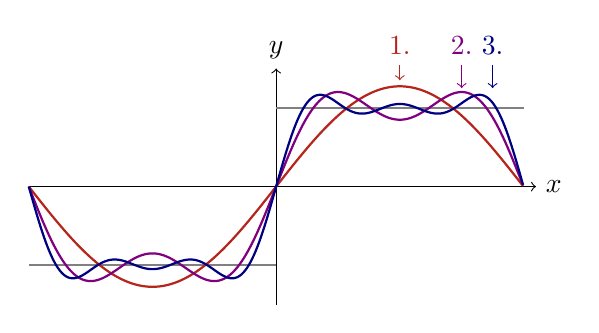
\begin{tikzpicture}
       \draw[->] (-pi,0) -- (3.3,0) node[anchor=west] {$x$};
       \draw[->] (0,-1.5) -- (0,1.5) node[anchor=south] {$y$};
       \draw[gray, thick] (-pi,-1) -- (0,-1); \draw[gray, thick] (0,1) -- (pi,1);
       \draw[thick,color=BrickRed] plot[domain=-pi:pi, samples=629] (\x, {(4/pi)*sin(180*\x/pi)});
       \draw[thick,color=Purple] plot[domain=-pi:pi, samples=629] (\x, {(4/pi)*(sin(180*\x/pi)+(1/3)*sin(180*3*\x/pi))});
       \draw[thick,color=NavyBlue] plot[domain=-pi:pi, samples=629] (\x, {(4/pi)*(sin(180*\x/pi)+(1/3)*sin(180*3*\x/pi))+(1/5)*sin(180*5*\x/pi))});
       \draw[<-, BrickRed] (pi/2, 1.35) -- +(0, .2) node[anchor=south]{\color{BrickRed}1.};
       \draw[<-, Purple] (3*pi/4, 1.25) -- +(0, .3) node[anchor=south]{\color{Purple}2.};
       \draw[<-, NavyBlue] (7*pi/8, 1.25) -- +(0, .3) node[anchor=south]{\color{NavyBlue}3.};
    \end{tikzpicture}
  } \medskip
  \caption{{\color{BrickRed}Erste}, {\color{Purple}zweite} and {\color{NavyBlue}dritte} 
  Fourier-Näherungen einer Rechtecksschwingung als Beispiel für eine Grafik\label{fig:tikz_fn}}
\end{figure}
}
\newcommand{\FHJExampleFigEN}{
\begin{figure}[!ht]
  \centerline{
    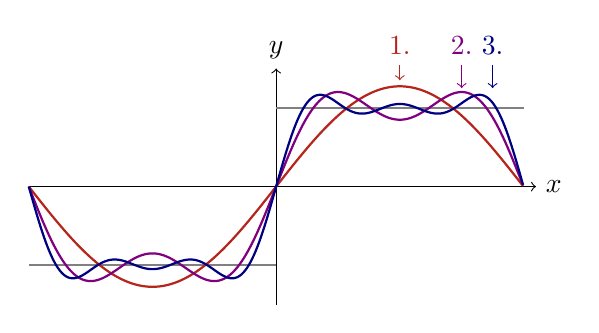
\begin{tikzpicture}
       \draw[->] (-pi,0) -- (3.3,0) node[anchor=west] {$x$};
       \draw[->] (0,-1.5) -- (0,1.5) node[anchor=south] {$y$};
       \draw[gray, thick] (-pi,-1) -- (0,-1); \draw[gray, thick] (0,1) -- (pi,1);
       \draw[thick, BrickRed] plot[domain=-pi:pi, samples=629] (\x, {(4/pi)*sin(180*\x/pi)});
       \draw[thick, Purple] plot[domain=-pi:pi, samples=629] (\x, {(4/pi)*(sin(180*\x/pi)+(1/3)*sin(180*3*\x/pi))});
       \draw[thick, NavyBlue] plot[domain=-pi:pi, samples=629] (\x, {(4/pi)*(sin(180*\x/pi)+(1/3)*sin(180*3*\x/pi))+(1/5)*sin(180*5*\x/pi))});
       \draw[<-, BrickRed] (pi/2, 1.35) -- +(0, .2) node[anchor=south]{\color{BrickRed}1.};
       \draw[<-, Purple] (3*pi/4, 1.25) -- +(0, .3) node[anchor=south]{\color{Purple}2.};
       \draw[<-, NavyBlue] (7*pi/8, 1.25) -- +(0, .3) node[anchor=south]{\color{NavyBlue}3.};
    \end{tikzpicture}
  } \medskip
  \caption{{\color{BrickRed}First}, {\color{Purple}second} and {\color{NavyBlue}third} nontrivial Fourier
    approximation of a square wave as an example for function plotting\label{fig:tikz_fn}}
\end{figure}
}
\newcommand{\FHJExampleTabDE}{
  \begin{table}[!ht]
    \centerline{
      \begin{tabular}{ll}
        \textbf{Zahl} & \textbf{Symbol/Wert} \\
        neutrales Element der Addition & $0$ \\
        neutrales Element der Multiplication & $1$ \\
        Euler'sche Zahl & $\mathrm e = 2.71828\,18284\,\ldots$ \\
        Verhältnis von Kreisumfang zu Durchmesser & $\pi = 3.14159\,26535\,\ldots$ \\
        imaginäre Einheit & $\mathrm i$ \hspace{5mm}with\hspace{5mm}$\mathrm i^2=-1$
      \end{tabular}
    }
    \caption{Einige bemerkenswerte Zahlen\label{tab:numbers}}
  \end{table}
}
\newcommand{\FHJExampleTabEN}{
  \begin{table}[!ht]
    \medskip
    \centerline{\begin{tabular}{ll}
      \textbf{number} & \textbf{symbol/value} \\
      neutral element of addition & $0$ \\
      neutral element of multiplication & $1$ \\
      Euler's number, related to growth & $\mathrm e = 2.71828\,18284\,\ldots$ \\
      ratio of circumference to diameter & $\pi = 3.14159\,26535\,\ldots$ \\
      imaginary unit & $\mathrm i$ \hspace{5mm}with\hspace{5mm}$\mathrm i^2=-1$
    \end{tabular}}
    \caption{Some notable numbers\label{tab:numbers}}
  \end{table}
}
%</package>
%    \end{macrocode}
% 
% \Finale
% 
\endinput
